\documentclass[margin=0px]{article}

\usepackage{listings}
\usepackage[utf8]{inputenc}
\usepackage{graphicx}
\usepackage{float}
\usepackage[a4paper, margin=0.7in]{geometry}
\usepackage{amsthm}
\usepackage{amssymb}
\usepackage{t1enc}
\usepackage{fancyhdr}
\usepackage{setspace}

\onehalfspacing

\newenvironment{tetel}[1]{\paragraph{#1 \\}}{}

\pagestyle{fancy}
\lhead{\it{PTI BSc Záróvizsga tételek}}
\rhead{14. Alapvető algoritmusok}

\title{\textbf{{\Large ELTE IK - Programtervező Informatikus BSc} \vspace{0.2cm} \\ {\huge Záróvizsga tételek}} \vspace{0.3cm} \\ 14. Alapvető algoritmusok}
\author{}
\date{}

\begin{document}
\maketitle

\begin{tetel}{Alapvető algoritmusok és adatszerkezetek}
    Függvények aszimptotikus viselkedése, algoritmusok hatékonysága. Összehasonlító rendezések (beszúró, összefésülő, gyors- és kupacrendezés), maximális műveletigény alsó korlátja. Rendezés lineáris időben (bucket, leszámláló és radix rendezés). Adattömörítés (naiv, Huffman, LZW). Mintaillesztés (brute-force, quicksearch, KMP).
\end{tetel}

\section{Függvények aszimptotikus viselkedése, algoritmusok hatékonysága}
TODO

\section{Összehasonlító rendező algoritmusok (buborék és beszúró rendezés, ill. verseny, kupac, gyors és összefésülő rendezés)}

Buborék- és beszúró rendezés klasszikusak, $n^2$-es műveletigényűek, a többi hatékony, $n\log(n)$-es idejűek.

\subsection{Buborékrendezés}

A legnagyobb értéket cserékkel a végéig felbuborékozza, ezt minden ciklus végén elhagyjuk. A gyakorlatban nem használják.
\begin{figure}[H]
    \centering
    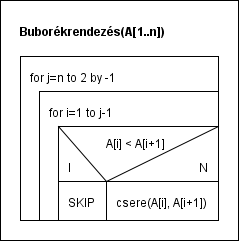
\includegraphics[width=0.3\textwidth]{img/Buborekrendezes.png}
    \caption{Buborékrendezés}
\end{figure}

\subsection{Beszúró rendezés}

Kis $n$-re (kb 30) ez a rendezés a legjobb. \\
Itt az elemmozgatás mindig 1 értékadás (buborékrendezésnél a csere 3 értékadás). Listára is implementálni lehet, ez esetben a pointereket állítjuk át, az elemek helyben maradnak. \\
$A[1..j]$ rendezett, $j=1..n$.
\begin{figure}[H]
    \centering
    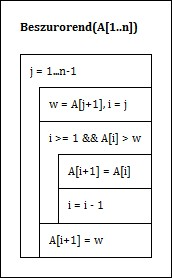
\includegraphics[width=0.3\textwidth]{img/Beszurorend.jpg}
    \caption{Beszúró rendezés}
\end{figure}

\subsection{Versenyrendezés}

Gyakorlatban nem használják. \\
Teljes bináris fa az alapja, egy versenyfa. Szintfolytonosan ábrázoljuk tömbösen.\\
\begin{enumerate}
    \item A versenyfa kitöltése (a verseny lejátszása). Maximum a gyökérben, ennek kiírása az outputra.
    \item $(n-1)$-szer
          \begin{itemize}
              \item[a)] gyökérben szereplő maximális elem helyének megkeresése a levélszinten és $-\infty$ írása a helyére
              \item[b)] az egészet újrajátsszuk (azt az ágat, ahol volt) $\to$ 2. legjobb feljut a gyökérbe
          \end{itemize}
\end{enumerate}
\begin{figure}[H]
    \centering
    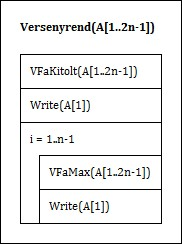
\includegraphics[width=0.3\textwidth]{img/Versenyrend.jpg}
    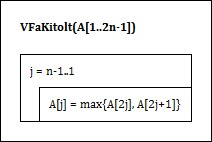
\includegraphics[width=0.3\textwidth]{img/VFaKitolt.jpg}
    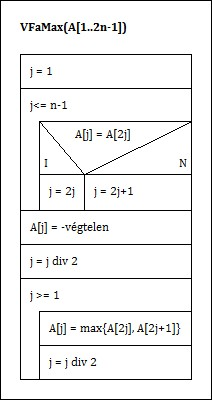
\includegraphics[width=0.3\textwidth]{img/VFaMax.jpg}
    \caption{Versenyrendezés}
\end{figure}

\subsection{Kupacrendezés}

\begin{enumerate}
    \item Kezdő kupac kialakítása. Rendezetlen input tömbből tartalmi invariánst készítünk, ami már kupac struktúrájú. Elv: cserékkel lesüllyesztjük az elemet a nagyobb gyerek irányába, ha kisebb a nagyobbik gyereknél. A süllyesztés eljuthat ahhoz a csúcshoz, amelynek nincs jobb gyereke.
    \item $(n-1)$-szer
          \begin{itemize}
              \item[a)] gyökérelem és az alsó szint jobb szélső (=utolsó) aktív elemének cseréje, és a csere után lekerült elem inaktívvá tétele
              \item[b)] a gyökérbe került elem süllyesztése az aktív kupacon
          \end{itemize}
\end{enumerate}
\begin{figure}[H]
    \centering
    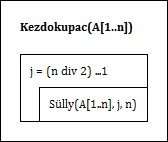
\includegraphics[width=0.3\textwidth]{img/Kezdokupac.jpg}
    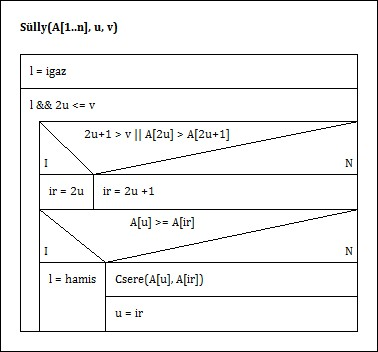
\includegraphics[width=0.3\textwidth]{img/Sully.jpg}
    \includegraphics[width=0.3\textwidth]{img/KupacRend.jpg}
    \caption{Kupacrendezés}
\end{figure}

A kezdőkupac kialakításánál, és a ciklus közben a süllyesztés módja kicsit különbözik, hiszen az első esetben a változó elem süllyed le a teljes kupacon, a másodikban a gyökér süllyed az aktív kupacon. A képen látható algoritmus mindkét műveletet teljesíti.

\subsection{Gyorsrendezés}

Elve: véletlenül választunk egy elemet. A nála kisebb elemeket tőle balra, a nagyobbakat jobbra rakjuk, az elemet berakjuk a két rész közé. Rekurzív algoritmus.
\begin{figure}[H]
    \centering
    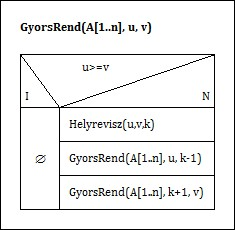
\includegraphics[width=0.3\textwidth]{img/GyorsRend.jpg}
    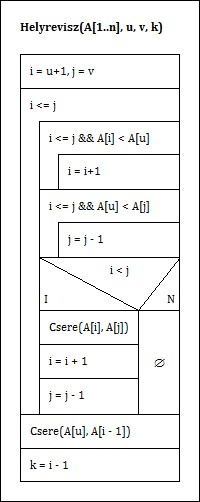
\includegraphics[width=0.3\textwidth]{img/Helyrevisz.jpg}
    \caption{Gyorsrendezés}
\end{figure}

\subsection{Összefésülő rendezés}

Alapja: 2 rendezett sorozat összefésülése. Ezt alkalmazhatjuk felülről lefelé (rekurzív) vagy alulról felfelé (iteratív), ez utóbbit szekvenciális fájloknál.
\begin{figure}[H]
    \centering
    \includegraphics[width=0.3\textwidth]{img/OFRend.jpg}
    \caption{Összefésülő rendezés}
\end{figure}

\section{A műveletigény alsó korlátja összehasonlító rendezésekre}

\subsection{Műveletigény}

Kijelöljük a domináns műveleteket, és az $n$ inputméret függvényében hányszor hajtódnak végre, ezt nézzük. Jelölés általánosan $T(n)$, de lehet konkrétan is, pl $Cs(n)$ [csere]. $mT(n)$ a minimális műveletigény, $MT(n)$ a maximális és $AT(n)$ az átlagos.
\begin{itemize}
    \item[$\Theta$]: nagyságrendileg azonos, két konstans közé beszorítható
    \item[$\mathcal{O}$]: nagyságrendi felső becslés, $o$: nincs megengedve az egyenlőség
    \item[$\Omega$]: nagyságrendi alsó becslés, $\omega$: nincs megengedve az egyenlőség
\end{itemize}

\subsection{Alsókorlát}

Például: $n$ elem maximumkiválasztása legalább $(n-1)$ összehasonlítást igényel. Bizonyítása: Ha ennél kevesebb összehasonlítás lenne, akkor legalább 1 elem kimaradt, és ezzel ellentmondásba kerülhetünk. \\
\textit{Döntési fa}: Algoritmus $n$ méretű inputra. Kiegyenesednek a ciklusok véges hosszú lánccá, a végrehajtás nyoma egy fa struktúrát ad. Tökéletes fa: minden belső pontnak 2 gyereke van. Ennél az algoritmusnál nincs jobb, mert $2^{h(t)} \geq n!$, összehasonlító rendezés esetén, $n!$ input.

\subsection{Alsókorlát legrosszabb esetben}

Tétel: $MO_R(n) = \Omega(n\log{n})$ A legkedvezőtlenebb permutációra legalább $n\log{n}$ összehasonlítás. Bizonyítás: $\log_2{n!} \leq n\log_2{n} = \Omega(n\log{n})$, és $MO_R(n)=h(t) \geq \log_2{n!}$ (lemma miatt) $\Rightarrow$ $MO_R(n)=\Omega(n\log{n})$.

\subsection{Alsókorlát átlagos esetben}

Legyen minden input egyformán valószínű ($\frac{1}{n!}$). \\
$AO_R(n) = \frac{1}{n!}\sum_{p \in Perm(n)}{O_R(p)}$, és könnyű belátni, hogy $\sum_{p}{O_R(p)} = lhsum(h(t_R(n)))$ [levél-magasság-összeg]. \\
Lemma: Az $n!$ levelet tartalmazó tökéletes fák közül azokra a legkisebb az $lhsum(h(t_R(n)))$ érték, amelyek majdnem teljesek. \\
Tétel: $AO_R(n) = \Omega(n\log{n})$.

\section{Rendezés lineáris időben (bucket-, leszámláló- és radix rendezés)}
TODO

\section{Adattömörítések}
\subsection{Naiv adattömörítés}
TODO

\subsection{Huffman-algoritmus}
A Huffman-algoritmussal való tömörítés lényege, hogy a gyakrabban előforduló elemeket (karaktereket) rövidebb, míg a ritkábban előfordulókar hosszabb kódszavakkal kódoljuk.

Ehhez tisztában kell lennünk az egyes karakterek gyakoriságával (vagy relatív gyakoriságával). Ezek alapján  egy ún. Huffman-fát építünk, melyben az éleket a kód betűivel címkézzük, a fa levelein a kódolandó betűk helyezkednek el, a gyökérből a levelekig vezető út címkéi alapján rajuk össze a kódszavakat.\\

\noindent
Az algoritmus (spec. bináris Huffman fára):
\begin{enumerate}
    \item A kódolandó szimbólumokat gyakoriságaik alapján sorba rendezzük.
    \item A következő redukciós lépéseket addig hajtjuk végre, míg egy csoportunk marad.
    \item Kiválasztjuk az utolsó két elemet (legritkább), összevonjuk őket egy új csoportba, és ennek a csoportnak a gyakorisága a gyakoriságok összege lesz.
    \item A csoportot visszahelyezzük a rendezett sorba (gyakoriság alapján rendezve).
    \item A csoportból új csúcsot képezünk, mely csúcs az őt alkotó két elem szülője lesz.
\end{enumerate}

\noindent
Példa:\\
Legyen a következő 5 betű, mely a megadott gyakorisággal fordul elő:\\

\begin{tabular}{|c|c|c|c|c|}
    \hline A & B & C & D & E \\
    \hline 5 & 4 & 3 & 2 & 1 \\
    \hline
\end{tabular}\\

Ekkor a redukciós lépések a következők:

\begin{itemize}
    \item \begin{tabular}{|c|c|c|c|}
              \hline A & B & C & D, E \\
              \hline 5 & 4 & 3 & 3    \\
              \hline
          \end{tabular}

    \item \begin{tabular}{|c|c|c|}
              \hline C, D, E & A & B \\
              \hline 6       & 5 & 4 \\
              \hline
          \end{tabular}

    \item \begin{tabular}{|c|c|}
              \hline A , B & C, D, E \\
              \hline 9     & 6       \\
              \hline
          \end{tabular}

    \item \begin{tabular}{|c|}
              \hline A , B , C, D, E \\
              \hline 15              \\
              \hline
          \end{tabular}
\end{itemize}

A huffman-fa a XY. ábrán látható.

\begin{figure}[H]
    \centering
    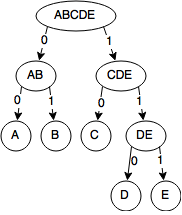
\includegraphics[width=0.3\textwidth]{img/Huffman_fa.png}
    \caption{Huffman-fa példa}
    \label{fig:Huffman_fa}
\end{figure}

Tehát a kódszavak:

\begin{tabular}{|c|c|c|c|c|}
    \hline A  & B  & C  & D   & E   \\
    \hline 00 & 01 & 10 & 110 & 111 \\
    \hline
\end{tabular}
\subsection{LZW-algoritmus}
Az LZW (Lempel-Ziv-Welch) tömörítésnek a lényege, hogy egy szótárat bővítünk folyamatosan, és az egyes kódolandó szavakhoz szótárindexeket rendelünk.
\begin{description}
    \item[Kódolás] \hfill \\
        A kódolás algoritmusa a következő lépésekből áll:
        \begin{enumerate}
            \item A szótárt inicializáljuk az összes 1 hosszú szóval
            \item \label{itm:szotar} Kikeressük a szótárból a leghosszabb, jelenlegi inputtal összeillő $W$ sztringet
            \item $W$ szótárindexét kiadjuk, és $W$-t eltávolítjuk az inputról
            \item A $W$ szó és az input következő szimbólumának konkatenációját felvesszük a szótárba
            \item A \ref{itm:szotar}. lépéstől ismételjük
        \end{enumerate}
    \item[Dekódolás] \hfill \\
        A dekódolás során is építenünk kell a szótárat. Ezt már azonban csak a dekódolt szöveg(rész) segítségével tudjuk megtenni, mivel egy megkapott kód dekódolt szava és az utána lévő szó első karakteréből áll össze a szótár következő eleme.

        Tehát a dekódolás lépései:
        \begin{enumerate}
            \item Kikeressük a kapott kódhoz tartozó szót a szótárból ($u$), az output-ra rakjuk
            \item Kikeressük a következő szót ($v$) a szótárból, az első szimbólumát $u$-hoz konkatenálva a szótárba rakjuk a következő indexszel.
            \item Amennyiben már nincs következő szó, dekódolunk, de nem írunk a szótárba.
        \end{enumerate}

        Megtörténhet az az eset, hogy mégis kapunk olyan kódszót, mely még nincs benne a szótárban. Ez akkor fordulhat elő, ha a kódolásnál az aktuálisan szótárba írt szó következik.\\

        Példa:

        Szöveg: AAA\\
        Szótár: A - 1

        Ekkor a kódolásnál vesszük az első karaktert, a szótárbeli indexe 1, ezt kiküldjük az outputra. A következő karakter A, így AA-t beírjuk a szótárba 2-es indexszel. Az első karaktert töröljük az inputról. Addig olvasunk, míg szótárbeli egyezést találunk, így AA-t olvassuk (amit pont az előbb raktunk be), ennek indexe 2, tehát ezt küldjük az outputra. AA-t töröljük az inputról, és ezzel végeztünk is. Az output: 1,2

        Dekódoljuk az 1,2 inputot! Jelenleg a szótárban csak A van 1-es indexszel. Vegyük az input első karakterét, az 1-et, ennek szótárbeli megfelelője A. Ezt tegyük az outputra. A következő index a 2, de ilyen bejegyzés még nem szerepel a szótárban. \\

        Ebben az esetben a dekódolásnál, egy trükköt vetünk be. A szótárba írás pillanatában még nem ismert a beírandó szó utolsó karaktere (A példában A-t találtuk, de nem volt 2-es bejegyzés). Ekkor ?-et írunk a szótárba írandó szó utolsó karakterének helyére. (Tehát A? - 2 kerül a szótárba). De mostmár tudni lehet az új bejegyzés első betűjét ( A? - 2 az új bejegyzés, ennek első betűje A). Cseréljük le a ?-et erre a betűre. (Tehát AA - 2 lesz a szótárban).
\end{description}
\section{Mintaillesztés}
\subsection{Brute-force mintaillesztés}
TODO

\subsection{Knuth-Morris-Pratt algoritmus}
A Knuth-Morris-Pratt eljárásnak a Brute-Force (hasonlítsuk össze, toljunk egyet, stb..) módszerrel szemben az az előnye, hogy egyes esetekben, ha a mintában vannak ismétlődő elemek, akkor egy tolásnál akár több karakternyit is ugorhatunk.

\begin{figure}[H]
    \centering
    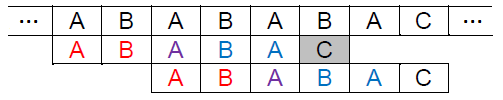
\includegraphics[width=0.4\textwidth]{img/KMP_sample.png}
    \caption{KMP algoritmus több karakter tolás estén}
    \label{fig:KMP_sample}
\end{figure}

Az ugrás megállapítását a következőképp tesszük: Az eddig megvizsgált egyező mintarész elején (prefix) és végén (suffix) olyan kartersorozatot keresünk, melyek megegyeznek. Ha találunk ilyet, akkor a mintát annyival tolhatjuk, hogy az elején lévő része ráilleszkedjen a végén levőre.

Azt, hogy ez egyes esetekben mekkorát tolhatunk nem kell minden elromlás alkalmával vizsgálni. Ha a mintára önmagával lefuttatjuk az algoritmus egy módosított változatát (\ref{fig:KMP_initnext}. ábra), kitölthetünk egy tömböt, mely alapján a tolásokat végezni fogjuk.

\begin{figure}[H]
    \centering
    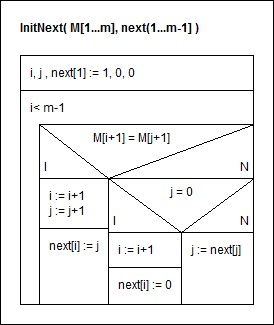
\includegraphics[width=0.3\textwidth]{img/KMP_initnext.jpg}
    \caption{KMP tolásokat szabályzó tömb kitöltése}
    \label{fig:KMP_initnext}
\end{figure}

Az algoritmus (ld \ref{fig:KMP}. ábra):
\begin{itemize}
    \item Két indexet $i$ és $j$ futtatunk a szövegen illetve a mintán.
    \item Ha az $i+1$-edik és $j+1$-edik karakterek megegyeznek, akkor léptetjük mind a kettőt.
    \item Ha nem egyeznek meg, akkor:
          \begin{itemize}
              \item Ha a minta első elemét vizsgáltuk, akkor egyet tolunk a mintán, magyarul a minta indexe marad az első betűn, és a szövegben lévő indexet növeljük eggyel ($i=i+1$)
              \item Ha nem a minta első elemét vizsgáltuk, akkor annyit tolunk, amennyit szabad. Ez azt jelenti, hogy csak a mintán lévő indexet helyezzük egy kisebb helyre ($j = next[j]$)
          \end{itemize}
    \item Addig megyünk, míg vagy a minta, vagy a szöveg végére nem érünk. Ha a minta végére értünk, akkor megtaláltuk a mintát a szövegben, ha a szöveg végére értünk, akkor pedig nem.
\end{itemize}

\begin{figure}[H]
    \centering
    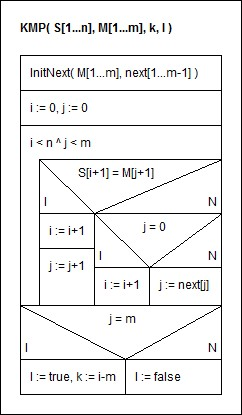
\includegraphics[width=0.3\textwidth]{img/KMP.jpg}
    \caption{KMP algoritmus}
    \label{fig:KMP}
\end{figure}
\subsection{Boyer-Moore  | Quick search algoritmus}
Míg a KMP algoritmus az elromlás helye előtti rész alapján döntött a tolásról, addig a QS a minta utáni karakter alapján. Tehát elromlás esetén:
\begin{itemize}
    \item Ha a minta utáni karakter benne van a mintában, akkor jobbról az első előfordulására illesztjük. (\ref{fig:BoyerMoore_shift1}. ábra)
          \begin{figure}[H]
              \centering
              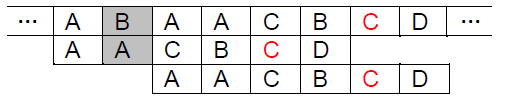
\includegraphics[width=0.4\textwidth]{img/BoyerMoore_shift1.png}
              \caption{QS - eltolás ha a minta utáni karakter benne van a mintában}
              \label{fig:BoyerMoore_shift1}
          \end{figure}
    \item Ha a minta utáni karakter nincs benne a mintában, akkor a mintát ezen karakter után illesztjük. (\ref{fig:BoyerMoore_shift2}. ábra)
          \begin{figure}[H]
              \centering
              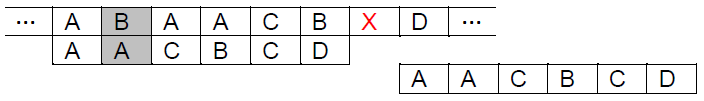
\includegraphics[width=0.6\textwidth]{img/BoyerMoore_shift2.png}
              \caption{QS - eltolás ha a minta utáni karakter nincs benne a mintában}
              \label{fig:BoyerMoore_shift2}
          \end{figure}
\end{itemize}

Az eltolás kiszámítását megint elő lehet segíteni egy tömbbel, most azonban, mivel nem a minta az érdekes, és nem tudjuk pontosan mely karakterek szerepelnek a szövegben, így a tömbbe az egész abc-t fel kell vennünk (\ref{fig:BoyerMoore_initshift}. ábra)

\begin{figure}[H]
    \centering
    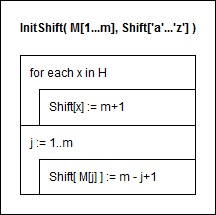
\includegraphics[width=0.3\textwidth]{img/BoyerMoore_initshift.jpg}
    \caption{QS - Az eltolást elősegítő tömb ($Shift['a'...'z']$) konstruálása}
    \label{fig:BoyerMoore_initshift}
\end{figure}

Az algoritmus (ld. \ref{fig:BoyerMoore}. ábra):
\begin{itemize}
    \item Két indexet $k$ és $j$ futtatunk a szövegen illetve a mintán.
    \item Ha a szöveg $k+j$-edik eleme megegyezik a minta $j$-edik karakterével, akkor léptetjük $j$-t (mivel a szövegben $k+j$-edik elemet nézzük, így elég $j$-t növelni).
    \item Ha nem egyeznek meg, akkor:
          \begin{itemize}
              \item Ha a minta már a szöveg végén van ($k=n-m$), akkor csak növeljük $k$-t eggyel, ami hamissá teszi a ciklus feltételt.
              \item Ha még nem vagyunk a szöveg végén $k$-t toljuk annyival, amennyivel lehet (ezt az előre beállított $Shift$ tömb határozza meg). És a $j$-t visszaállítjuk 1-re.
          \end{itemize}
    \item Addig megyünk, míg vagy a minta végére érünk $j$-vel, vagy a mintát továbbtoltuk a szöveg végénél. Előbbi esetben egyezést találtunk, míg az utóbbiban nem.
\end{itemize}

\begin{figure}[H]
    \centering
    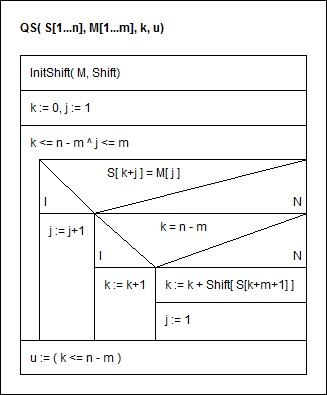
\includegraphics[width=0.4\textwidth]{img/BoyerMoore.jpg}
    \caption{QS}
    \label{fig:BoyerMoore}
\end{figure}
\subsection{Rabin-Karp algoritmus}
A Rabin-Karp algoritmus lényege, hogy minden betűhöz az ábécéből egy számjegyet rendelünk, és a keresést számok összehasonlításával végezzük. Világos, hogy ehhez egy ábécé méretnek megfelelő számrendszerre lesz szükségünk. A szövegből mindig a minta hosszával egyező részeket szelünk ki, és ezeket hasonlítjuk össze.\\

\noindent
Példa:\\
Minta: BBAC $\rightarrow$ 1102 \\
Szöveg: DACABBAC $\rightarrow$ 30201102, amiből a következő számokat állítjuk elő: 3020, 0201, 2011, 0110, 1102\\

\noindent
A fent látható szeletek lesznek az $s_i$-k.\\

\noindent
Az algoritmus működéséhez azonban számos apró ötletet alkalmazunk:
\begin{enumerate}
    \item A minta számokká alakítását Horner-módszer segítségével végezzük.
          \begin{figure}[H]
              \centering
              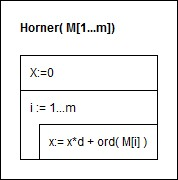
\includegraphics[width=0.3\textwidth]{img/RK_Horner.jpg}
              \caption{RK - Horner-módszer}
              \label{fig:RK_Horner}
          \end{figure}
          Az $ord()$ függvény az egyes betűknek megfelelő számot adja vissza. A $d$ a számrendszer alapszáma.
    \item A szöveg mintával megegyező hosszú szeleteinek ($s_i$) előállítása: \\
          $s_0$-t a Horner-módszerrel ki tudjuk számolni. Ezek után $s_{i+1}$ a következőképp számolandó:
          \[s_{i+1} = (s_i - ord(S[i])\cdot d^{m-1})\cdot d  + ord(S[i+1])\]
          \textit{Magyarázat: $s_i$ elejéről levágjuk az első számjegyet ($s_i - ord(S[i])\cdot d^{m-1}$), majd a maradékot eltoljuk egy helyiértékkel (szorzás $d$-vel), végül az utolsó helyiértékre beírjuk a következő betűnek megfelelő számjegyet ($+ord(S[i+1])$)}

          Példa:

          Az előző példa szövegével és mintájával ($d=10$ elemű ábécé és $m=4$ hosszú minta): \\
          $s_0 = 3020$, ekkor: $s_{0+1} = s_1 = (3020 - ord(D) \cdot 10^3)\cdot 10 + ord(B) = (3020-3000)\cdot 10 +1 = 0201$
    \item Felmerülhet a kérdés, hogy az ilyen magas alapszámú számrendszerek nem okoznak-e gondot az ábrázolásnál? A kérdés jogos. Vegyük a következő életszerű példát:

          4 bájton ábrázoljuk a számainkat ($2^{32}$). Az abc legyen 32 elemű ($d=32$), a minta 8 hosszú ($m=8$). Ekkor a $d^{m-1}$ kiszámítása: $32^7 = (2^5)^7 = 2^{35}$ , ami már nem ábrázolható 4 bájton.

          Ennek kiküszöbölésére vezessünk be egy nagy $p$ prímet, melyre $d\cdot p$ még ábrázolható. És a műveleteket számoljuk {\it mod p}. Ekkor természetesen a kongruencia miatt lesz olyan eset, amikor az algoritmus egyezést mutat, mikor valójában nincs. Ez nem okoz gondot, mivel ilyen esetben karakterenkénti egyezést vizsgálva ezt a problémát kezelni tudjuk. (Fordított eset nem fordul elő tehát nem lesz olyan eset, mikor karakterenkénti egyezés van, de numerikus nincs). [Ha $p$ kellően nagy, a jelenség nagyon ritkán fordul elő.]

    \item A {\it mod p} számítás egy másik problémát is felvet. Ugyanis a kivonás alkalmával negatív számokat is kaphatunk.

          Például: Legyen $p=7$, ekkor, ha $ord(S[i]) = 9$, akkor előző számítás után $s_i = 2...$, de ebből $ord(S[i])\cdot d^{m-1} = 9\cdot 10^3 = 9000$-et vonunk ki negatív számot kapunk.

          Megoldásként $s_{i+1}$-et két lépésben számoljuk:
          \[s := (s_i+d\cdot p - ord(S[i])\cdot d^{m-1}) \quad mod \quad p \]
          \[s_{i+1} := (s\cdot d + ord(S[i+1])) \quad mod \quad p \]
\end{enumerate}
A fentiek alapján az algoritmus a következő (ld. \ref{fig:RK}. ábra)
\begin{enumerate}
    \item Kiszámoljuk $d^{m-1}$-et ($dm1$)
    \item Egy iterációban meghatározzuk Horner-módszerrel a minta számait ($x$) és $s_0$-t
    \item Ellenőrizzük, hogy egyeznek-e
    \item Addig számolgatjuk $s_i$ értékét míg a minta nem egyezik $s_i$-vel, vagy a minta a szöveg végére nem ért.
\end{enumerate}
\begin{figure}[H]
    \centering
    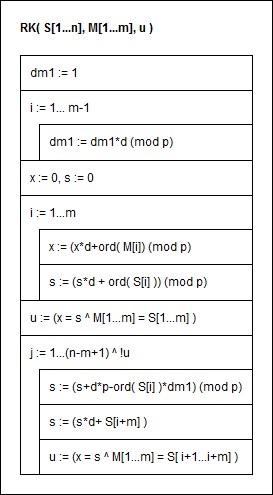
\includegraphics[width=0.3\textwidth]{img/RK.jpg}
    \caption{RK}
    \label{fig:RK}
\end{figure}

\end{document}